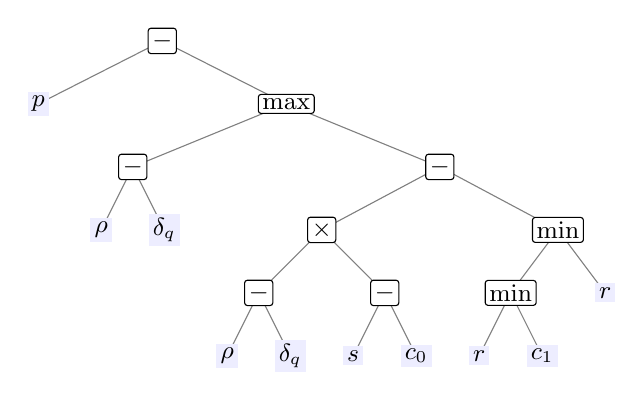
\begin{tikzpicture}[x=8mm,y=8mm,every node/.style={font=\small,inner sep=1.5pt}]
\draw[gray] (1.5,-2) -- (1,-3);
\draw[gray] (1.5,-2) -- (2,-3);
\draw[gray] (3.5,-4) -- (3,-5);
\draw[gray] (3.5,-4) -- (4,-5);
\draw[gray] (5.5,-4) -- (5,-5);
\draw[gray] (5.5,-4) -- (6,-5);
\draw[gray] (4.5,-3) -- (3.5,-4);
\draw[gray] (4.5,-3) -- (5.5,-4);
\draw[gray] (7.5,-4) -- (7,-5);
\draw[gray] (7.5,-4) -- (8,-5);
\draw[gray] (8.25,-3) -- (7.5,-4);
\draw[gray] (8.25,-3) -- (9,-4);
\draw[gray] (6.375,-2) -- (4.5,-3);
\draw[gray] (6.375,-2) -- (8.25,-3);
\draw[gray] (3.9375,-1) -- (1.5,-2);
\draw[gray] (3.9375,-1) -- (6.375,-2);
\draw[gray] (1.96875,0) -- (0,-1);
\draw[gray] (1.96875,0) -- (3.9375,-1);
\node[fill=blue!7] at (0,-1) {$p$};
\node[fill=blue!7] at (1,-3) {$\rho$};
\node[fill=blue!7] at (2,-3) {$\delta_q$};
\node[draw,rounded corners=1pt,fill=white] at (1.5,-2) {$-$};
\node[fill=blue!7] at (3,-5) {$\rho$};
\node[fill=blue!7] at (4,-5) {$\delta_q$};
\node[draw,rounded corners=1pt,fill=white] at (3.5,-4) {$-$};
\node[fill=blue!7] at (5,-5) {$s$};
\node[fill=blue!7] at (6,-5) {$c_{0}$};
\node[draw,rounded corners=1pt,fill=white] at (5.5,-4) {$-$};
\node[draw,rounded corners=1pt,fill=white] at (4.5,-3) {$\times$};
\node[fill=blue!7] at (7,-5) {$r$};
\node[fill=blue!7] at (8,-5) {$c_{1}$};
\node[draw,rounded corners=1pt,fill=white] at (7.5,-4) {$\min$};
\node[fill=blue!7] at (9,-4) {$r$};
\node[draw,rounded corners=1pt,fill=white] at (8.25,-3) {$\min$};
\node[draw,rounded corners=1pt,fill=white] at (6.375,-2) {$-$};
\node[draw,rounded corners=1pt,fill=white] at (3.9375,-1) {$\max$};
\node[draw,rounded corners=1pt,fill=white] at (1.96875,0) {$-$};
\end{tikzpicture}
